% !Mode:: "TeX:UTF-8"
% !TEX program  = xelatex
\documentclass[a4paper]{article}
\usepackage{amsmath}
\usepackage{amssymb}
\usepackage{ctex}
%\usepackage{braket}
%\usepackage[european]{circuitikz}
\usepackage{multirow}
\usepackage{float}
\usepackage{colortbl}
\usepackage{graphicx}
\usepackage{geometry}
\geometry{left=2.5cm,right=2.5cm,bottom=2.5cm,top=2.5cm}
\title{近代物理实验报告9.1:核磁共振}
\author{xy\quad 学号\quad 匡亚明学院}
\date{2019年2月29日}
\begin{document}
\maketitle
\bibliographystyle{unsrt}
%--------main-body------------

\section{引言}
1946年,美国斯坦福大学的Bloch等人和哈佛大学的Purcell等人独立地采用原子核感应法,即同时将一个恒定磁场和沿垂直于恒定磁场方向上的一个交变磁场同时作用于原子核系统上,然后测定由原子核磁矩进动所感应的电动势,发现了核磁共振现象。后来Bloch和Purcell因为这一发现而获得了1952年度的诺贝尔物理学奖。今天,核磁共振己成为研究物质结构和原子核的磁性、进行各种化合物的分析租鉴定、精密测定各种原子核磁矩以及作为核磁共振成像仪的重要原理和组成部分在医学上进行诊断的有力工具。

\section{实验仪器}
核磁共振仪。

\section{实验原理}
\subsection{原子核的基本特性}

原子由原子核和核外运动的电子所组成。原子核的电荷、质量、成分、大小、角动量和磁矩构成了它的的基本性质。众所周知,原子核带正电,所带电量和核外电子的总电量相等,数值上等于最小电量单位$e$(1.6021$\times $10$^{-19}$C)的整数倍,称为电荷数。原子核的质量一般用质量数表示,接近于原子质量单位(1.66055 $\times $10$^{-27}$kg)的整数倍。原子核由质子和中子所组成。质子和中子的质量大致相等,但每个质子带正电量$e$,而中子则不带电。因此,元素周期表中的原子序数$Z$在数值上等于相应原子核外的电子数、核内质子数和核的电荷数。原子核的半径为10$^{-15}$m的数量级。

原子核具有本征角动量,通常称为原子核的自旋,等于核内所有轨道和自旋运动的角动量的总和。核自旋可用自旋量子数I来表征。核内的中子和质子都是$I$=1/2的粒子。实验证明,如将原子核按其自旋特性来分类,则可分为三类:(1)电荷数(即原子序数)与质量数都为偶数的核,如$^{12}$C,$^{18}$O)等,它们的自旋量子数为零;(2)质量数为单数的核,如$^1$H,$^{13}$C,$^{15}$N等,它们的自旋量子数为半整数(1/2,3/2,5/2);(3)质量数为双数,但电荷数(原子序数)为单数的核,$^2$H,$^{14}$N等,它们的自旋量子数为整数(1,2,3,...)。

根据量子力学,一自旋量子数$I\neq0$的孤立原子核应具有本征自旋角动量$P_I$和本征自旋磁矩$\mu_I$:

$$P_I=\sqrt{I(I+1)\hbar},\mu_I=g_l\sqrt{I(I+1)\mu_N},$$

$P_I$和$\mu_I$方向互相平行。式中,$g_I$为原子核的朗德分裂因子,即$g$因子,其值随原子核的不同而不同。$\mu_N=\frac{e\hbar}{2M_P}=5.050824\times 10^{-27}\text{J/T}$,称为核磁子,是核磁矩的单位。这里的$e$和$M_P$分别是质子的电荷与质量。和电子磁矩的单位——玻尔磁子$\mu_B$相比($\mu_B=\frac{e\hbar}{2m_e}=9.204078\times 10^{-24}\text{J/T}$,$e$和$m_e$分别是电子的电荷和质量),因为电子质量仅为质子质量的1/1360,可知$\mu_B$比$\mu_N$要大得多,因而,电子磁矩也要比原子核磁矩大得多。原子核的磁矩可正可负,例如经测定,以$\mu_N$为单位,中子($^1$n,$I=1/2$)和$^{17}$O的磁矩都为负值,分别为-1.9130和-1.8930,而质子($^{1}$H,$I=1/2$)和$^{13}\text{C}$,$I=1/2$的磁矩均为正值,分别为2.7927和0.7022。

现在,设想一原子核位于沿$z$方向施加的恒定磁场$H_0$中,由于空间量子化,$P_I$和$\mu_I$沿$z$方向的分量$P_z$,$\mu_z$只能取一系列不连续的值:
$$P_z=m\hbar,$$
$$\mu_z=\gamma'P_z=m\gamma'\hbar.$$
式中,$\gamma'$是核磁矩和核自旋角动量之比,称为核的旋磁比;$m$是磁量子数,可取$I$,$I-1$,$I-2$,...,$-I+1$,$-I$等共$2I+1$个不连续的值。

应该指出,人们通常所说的原子核的角动量和磁矩指的是$P_z$,$\mu_z$的最大值,即
$$P=(P_z)_\text{max}=I\hbar,$$
$$\mu=(\mu_z)_\text{max}=\gamma'I\hbar.$$

\subsection{核磁共振的经典物理描述}

从经典物理的观点看,如果定义单位体积内原子核磁矩的矢量和磁化强度为$\mathbf{M}$,则当该原子核系统位于恒定磁场中时,$\mathbf{M}$将以一定的角速度围绕磁场轴作拉莫(Lamor)进动并最终沿磁场方向取向。如图\ref{Fig1}(a)所示,这一过程涉及外加磁场作用下的自旋动力学问题。根据刚体转动力学原理,一绕自身轴转动的刚体(如陀螺)在受到一外力矩作用时,该刚体除了自身转动外,其自转轴还会绕着外力方向作进动。将原子核自旋系统与这种刚体的行为作类比,可以容易地写出无阻尼振动的理想情况下,该系统的角动量随时间的变化率应等于外加的磁场力矩,即
$$\frac{{\rm d}\mathbf{P}}{{\rm d}t}=\mu_0\mathbf{M}\times \mathbf{H}.$$
考虑到$M=\gamma'P$,可得原子核磁矩的进动方程为
$$\frac{{\rm d}\mathbf{M}}{{\rm d}t}=\gamma\mathbf{M}\times \mathbf{H}.$$
式中,$\gamma=\mu_0\gamma'=\frac{\mu_0eg_I}{2M_N}$表示核的磁偶极矩与自旋角动量比值的旋磁比。$\mu_0$和$M_N$分别是真空磁导率($\mu_0=4\pi\times 10^{-7}\text{H/m}$)和核的质量。核磁矩的进动图像如图\ref{Fig1}(a)所示,${\rm d}\mathbf{M}/{\rm d}t$垂直于$\mathbf{M}-\mathbf{H}$平面,使$\mathbf{M}$绕$\mathbf{H}$进动。

设在${\rm d}t$时间内$\mathbf{M}$从点$A$进动到点$B$,相应的$\theta$角保持不变,而在$x-y$平面内角度改变${\rm d}\varphi$,从图中几何关系可知${\rm d}M=\overline{AB}=M\sin\theta{\rm d}\varphi$,由此可得$\mathbf{M}$的拉莫进动频率为
$$\omega=\frac{{\rm d}\varphi}{{\rm d}t}=\frac{1}{M\sin\theta}\frac{{\rm d}M}{{\rm d}t}=\frac{\gamma MH\sin\theta}{M\sin\theta}=\gamma H.$$

\begin{figure}[H]
\centering
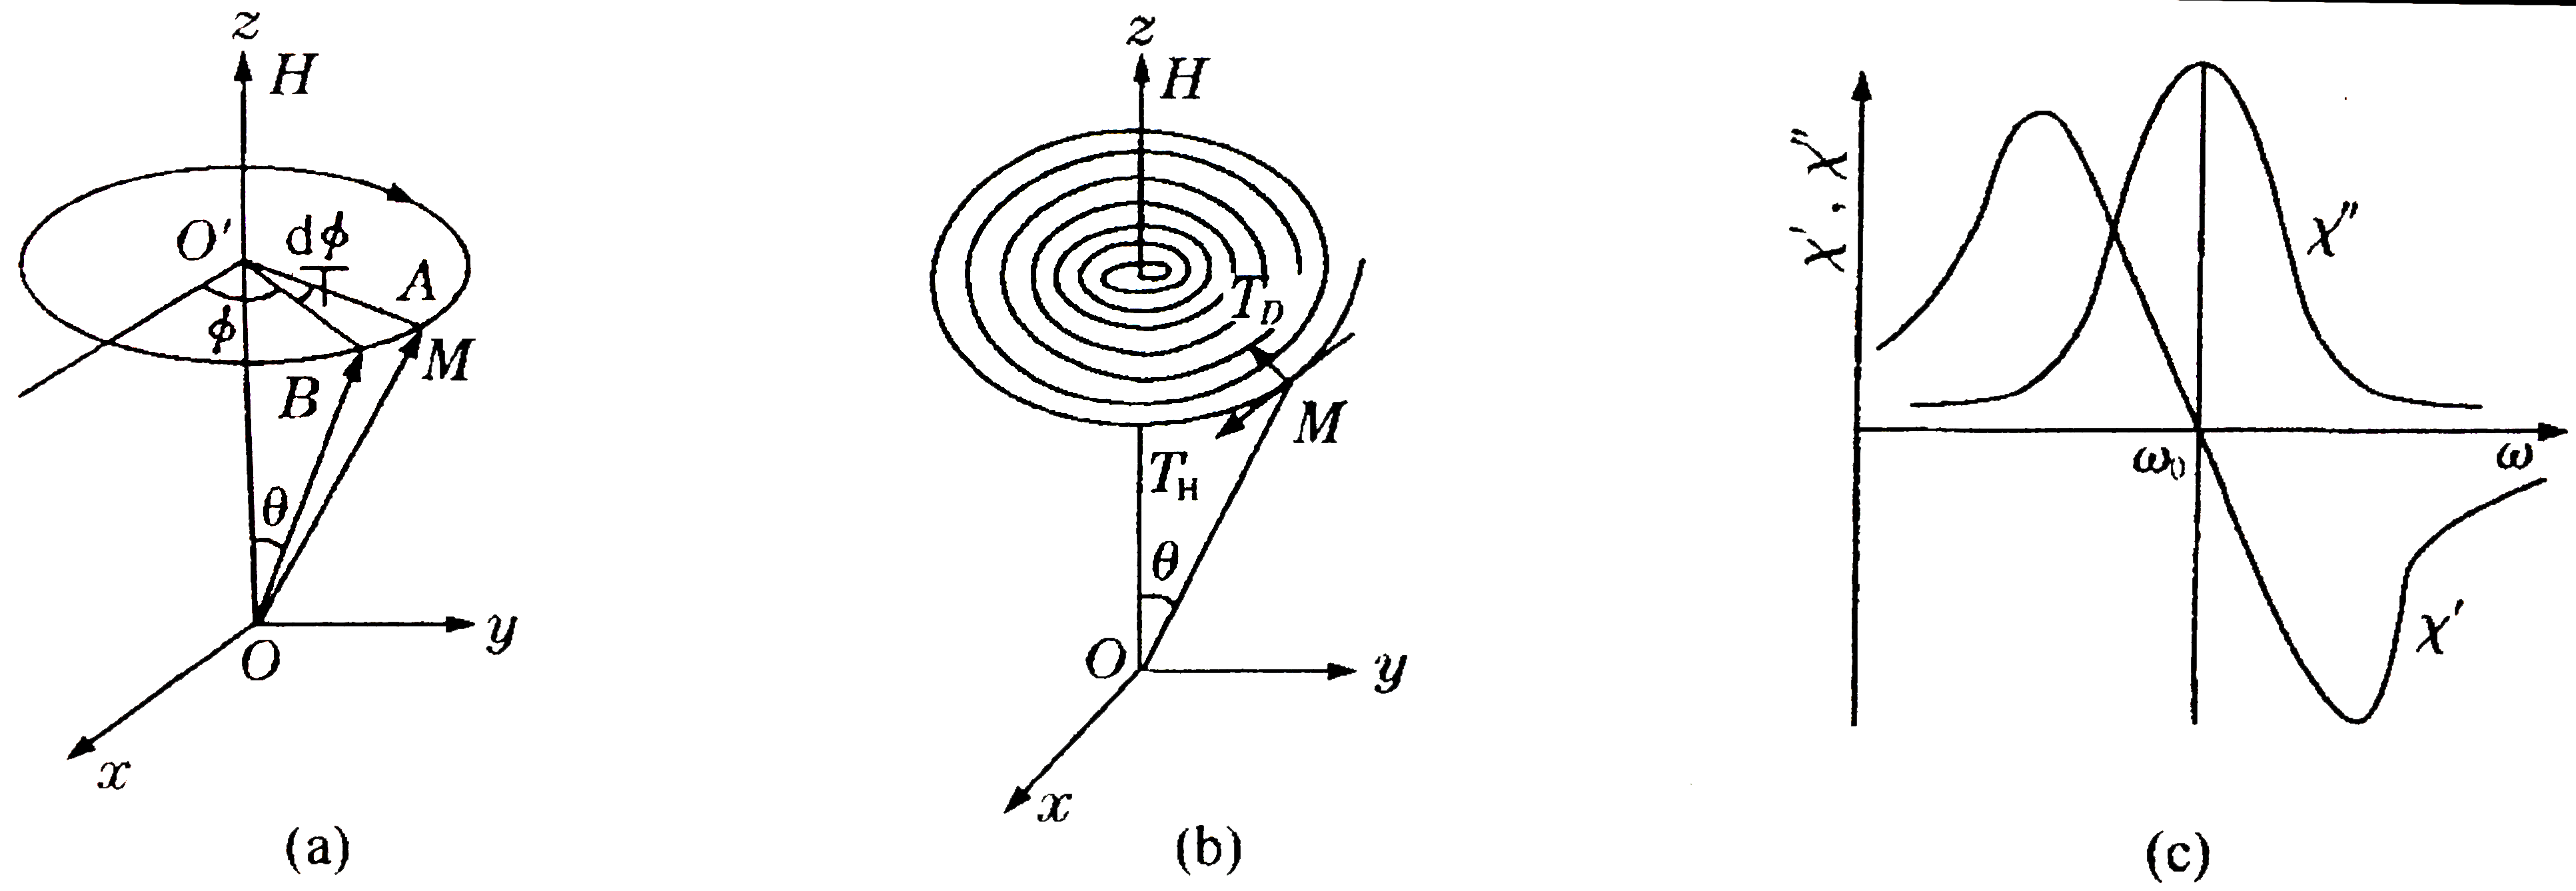
\includegraphics[width = 0.8\textwidth]{fig/1.png}\\
\caption{原子核自旋磁矩在外磁场中的拉莫进动和核磁共振的经典描述}
\label{Fig1}
\end{figure}

在实际情况下,$\mathbf{M}$绕$\mathbf{H}$进动会受到阻尼作用,因而随着进动的进行,$\mathbf{M}$与$\mathbf{H}$之间的夹角$\theta$将随时间而减小,最后达到位置平衡,使$\mathbf{M}$平行于$\mathbf{H}$取向,如图\ref{Fig2}(a)所示,为了描述这一物理图像,可通过唯象地再同时引入一阻尼力矩$\mathbf{T}_D$,推导出下列进动方程:
\begin{equation}\frac{{\rm d}\mathbf{M}}{{\rm d}t}=\gamma\mathbf{M}\times \mathbf{H}+\mathbf{T}_D.\label{9.1-1}\end{equation}
阻尼力矩$\mathbf{T}_D$通常有三种表达式,即
\begin{equation}\text{Landau-Lifshitz形式:}\mathbf{T}_D=-\frac{4\pi\lambda}{M^2}\mathbf{M}\times (\mathbf{M}\times \mathbf{H})=-\frac{\alpha\gamma}{M}\mathbf{M}\times (\mathbf{M}\times \mathbf{H})\label{9.1-2}\end{equation}
\begin{equation}\text{Gilbert形式:}\mathbf{T}_D=\frac{\alpha}{M}\mathbf{M}\times \frac{{\rm d}\mathbf{M}}{{\rm d}t}\label{9.1-3}\end{equation}
\begin{equation}\text{Bloch形式:}\mathbf{T}_D=-\frac{M_x}{T_2}\mathbf{i}-\frac{M_y}{T_2}\mathbf{j}-\frac{M_z-M_0}{T_1}\mathbf{k}\label{9.1-4}\end{equation}
以上公式中,$\lambda>0$,它是一个同阻尼力矩大小有关系的系数,量纲是时间的倒数,称为弛豫频率。$\alpha$是阻尼系数,$T_1$和$T_2$分别称为自旋-自旋(纵向)弛豫时间和自旋-晶格(横向)弛豫时间,通常,$T_2\le T_1$。在实际使用中,用Landau-Lifshitz形式处理自旋动力学问题时非常方便,因而使用最多,但是,当$\lambda$很大时,会出现矛盾。Gilbert形式在数学处理上最为简单,Bloch形式能对人体内所有核磁共振现象给出非常满意的描述,所以多在医学上讨论核磁共振原理和信号处理时被应用。

现在,考察一下核自旋系统在恒定磁场和交变磁场共同作用下的响应。如果沿$+z$方向施加一恒定磁场$\mathbf{H}_0$,沿$+x$方向施加一弱交变磁场$\tilde{h}=h_0{\rm e}^{j\omega t}$,且满足$h_0<<H_0$。将下列条件代入\ref{9.1-1}和\ref{9.1-2}式,得
$$\mathbf{H}=h_0{\rm e}^{j\omega t}\mathbf{i}+H_0\mathbf{k},$$
$$\mathbf{M}=m_{x0}{\rm e}^{j\omega t}\mathbf{j}+(M_0-m_{z0}{\rm e}^{j\omega t})\mathbf{k}$$
忽略二级小量,考虑到$h_0<<H_0$,近似有$\frac{{\rm d}m_z}{{\rm d}t}\sim0$,同时令$\omega_0=\gamma H_0$,$\omega_c=\frac{4\pi\lambda}{\chi_0}$,$\chi_0=\frac{M_0}{H_0}$,可得联立方程组如下:
\begin{equation}(\omega_c+j\omega)m_{x0}-\omega_0m_{y0}=\omega_c\chi_0h_0,\label{9.1-5}\end{equation}
\begin{equation}\omega_0m_{x0}+(\omega_c+jw)m_{y0}=\gamma M_0h_0.\label{9.1-6}\end{equation}
解方程,可得沿$x$轴方向的磁化强度分量为
\begin{equation}m_{x0}=\frac{\omega_c^2+\omega_0^2+j\omega\omega_c}{\omega_c^2-\omega^2+\omega_0^2+2j\omega\omega_c}\chi_0h_0.\label{9.1-7}\end{equation}
由此可以求得复数交流磁化率$\tilde{\chi}=\frac{m_{x0}}{h_0}$,如果将该磁化率写成$\tilde{\chi}=\chi'-j\chi''$,经整理可得该复量磁化率的实部和虚部的表达式:
\begin{equation}\chi'=\frac{(\omega_c^2+\omega_0^2)^2+\omega^2(\omega_c^2-\omega_0^2)}{(\omega_c^2-\omega^2+\omega_0^2)^2+4\omega^2\omega_c^2}\chi_0,\label{9.1-8}\end{equation}
\begin{equation}\chi''=\frac{\omega\omega_c(\omega_c^2+\omega_0^2+\omega^2)}{(\omega_c^2-\omega^2+\omega_0^2)^2+4\omega^2\omega_c^2}\chi_0.\label{9.1-9}\end{equation}
图\ref{Fig1}(c)示出了阻尼(即\ref{9.1-2}式中的$\lambda$值)很小时$\chi'$和$\chi''$随角频率$\omega$的变化关系。可以看到,当弱交变磁场的频率等于拉莫进动的频率即$\omega=\omega_0=\gamma H_0$时,$\chi'$发生从正值到负值的突变,而$\chi''$则达到峰值,这正好对应于核磁共振发生的情况。复数磁化率的物理意义在于其实部代表系统中储存的能量,而虚部则代表能量损耗。位于交变磁场中的单位体积原子核自旋磁矩系统将以一定速率从该磁场中吸收能量,每一周期$T=\frac{2\pi}{\omega}$中所吸收的能量为
\begin{equation}E=\mu_0\int_{t=0}^{t=T}\mathbf{H}\cdot{\rm d}\mathbf{M}.\label{9.1-10}\end{equation}
因为只有$h\frac{{\rm d}m_x}{{\rm d}t}$项对上式积分有贡献,因此,如果沿$x$方向的交变磁场写成$h=h_0\cos\omega t$,则$m_x$为复数意味着其实部和$h$同相位,而虚部落后于$h$的相位角为$\pi/2$,于是$m_x$可写成
$$m_x=\chi'h_0\cos\omega t+\chi''h_0\cos(\omega t-\pi/2)=\chi'h_0\cos\omega t+\chi''h_0\sin\omega t.$$
代入\ref{9.1-8}式,积分后求得
\begin{equation}E=\pi\mu_0h_0^2\chi''.\label{9.1-11}\end{equation}
由此可知,单位体积核自旋系统每周从交变磁场中吸收的能量和交流磁化率的虚部成正比,图\ref{Fig1}(c)所示的$\chi''-\omega$关系反映了在实验上观察到的核磁共振峰的主要特点。

应该指出的是,在常见的核磁共振仪中,感生电动势是从一个垂直于交变磁场和恒定磁场放置的探测线圈中测得的。因此,实验时实际测量的是分量$m_y=m_{y0}{\rm e}^{j\omega t}$,从联立方程式\ref{9.1-5}和\ref{9.1-6}很容易求得
\begin{equation}m_{y0}=\frac{2\omega^2\omega_0\omega_c+j\omega\omega_0(\omega_c^2-\omega^2+\omega_0^2)}{(\omega_c^2-\omega^2+\omega_0^2)^2+4\omega^2\omega_c^2}\chi_0h_0.\label{9.1-12}\end{equation}

\subsection{}
氢原子核($^1$H)在有机化合物中占有很重要的地位。它对磁场的敏感度最大,容易观察到满意的核磁共振信号,因而目前对它的研究最多,应用也最广泛。

氢原子核只包含一个质子,自旋量子数为$I=1/2$,可以看成是电荷均匀分布于球面上的旋转椭球。在恒定磁场中,它有平行和反平行于磁场两种取向,相应于$m=+1/2$和$m=-1/2$。这两种取向的能量是不同的,用两个能级来表示,如图\ref{Fig2}所示。其中,$m=-1/2$能级因自旋取向与磁场方向相反,能量较高,这两个能级之间的能量差为
$\Delta E=\gamma_P\hbar H_0,$
式中,$\gamma_P=3.36166\times 10^2/$(A/M$\cdot$sec)是质子的旋磁比。

\begin{figure}[H]
\centering
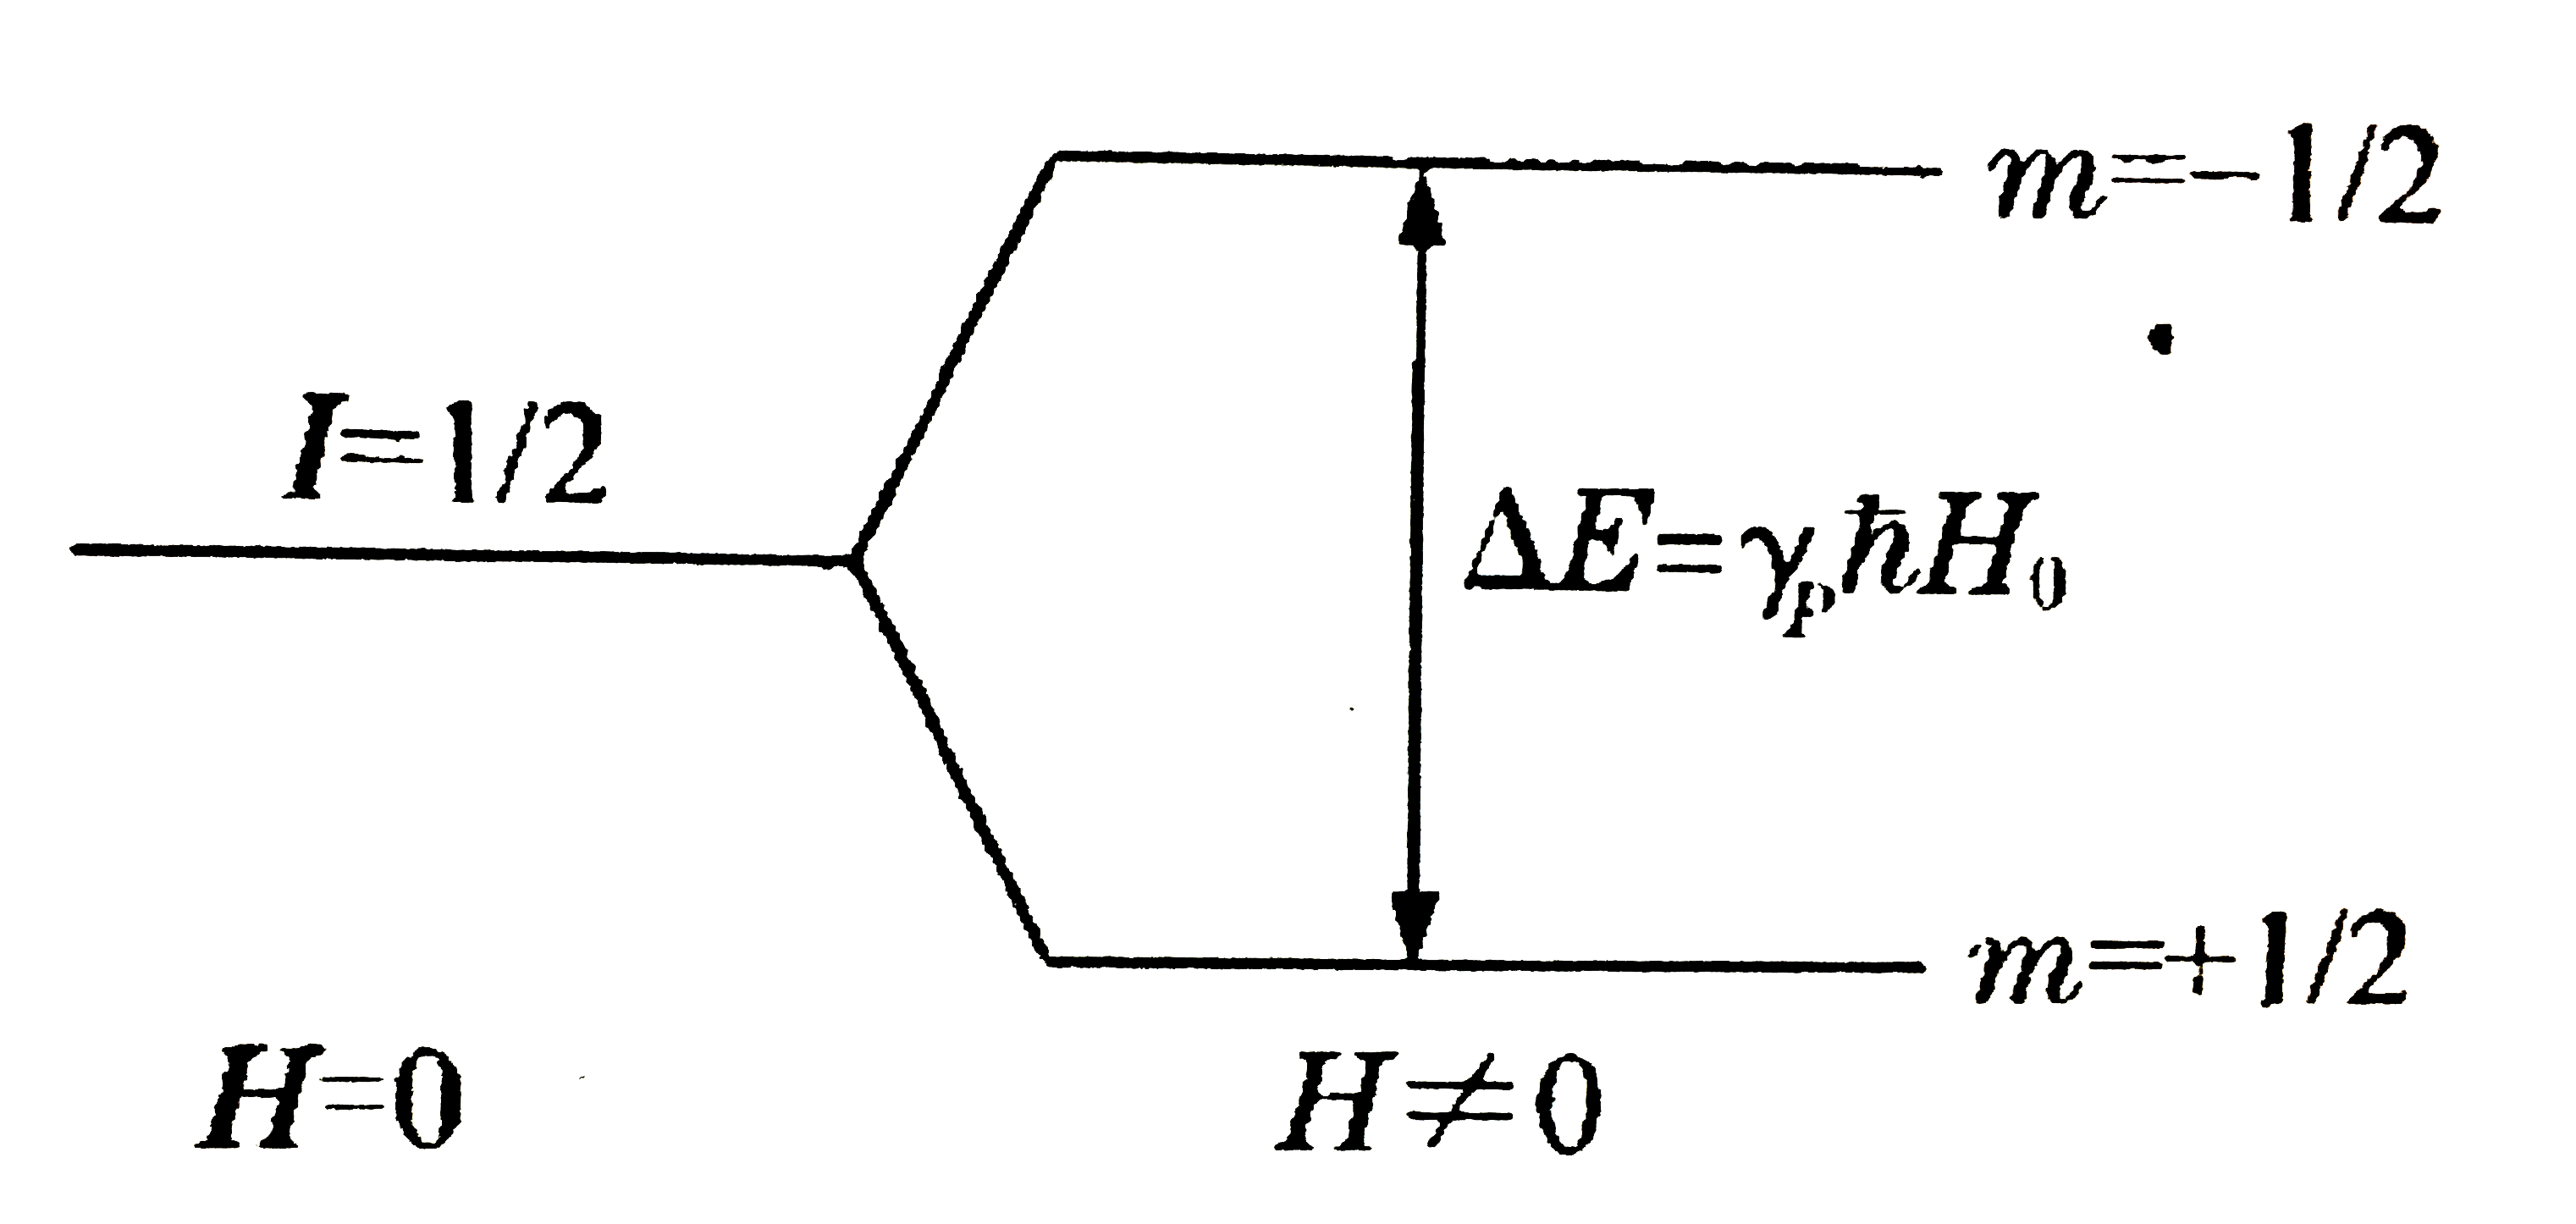
\includegraphics[width = 0.5\textwidth]{fig/2.png}\\
\caption{氢原子自旋磁矩在恒定磁场中的能积分裂}
\label{Fig2}
\end{figure}

可由统计力学估算出热平衡条件下$m=+1/2$的质子数$N_+$与$m=-1/2$的质子数$N_-$之比:
\begin{equation}\frac{N_+}{N_-}=\exp\left(\frac{\Delta E}{kT}\right)=\exp\left(\frac{\gamma_0\hbar H_0}{kT}\right)\approx 1+\frac{\gamma_0 \hbar H_0}{kT}.\label{9.1-13}\end{equation}
假定$H_0=1.1214\times 10^3$kA/m(14902Oe),$T=300$K(这是60MHz核磁共振仪室温下测量的典型条件),则$N_+/N_-=1.0000099$,这就是说,在一百万个氢原子核中,热平衡条件下位于低能级的原子核数只比位于高能级的多10个左右。

如果要使位于低能级的核跃迁到较高能级去,即从$m=+1/2$的能级跃迁到$m=-1/2$的能级,就必须向原子核提供正好等于两个能级之间的能量差$\Delta E$的电磁波能量。如果在垂直于恒定磁场$H_0$的方向上对氢原子核系统施加一个角频率为$\omega_0$的交变磁场,其提供的能量$\hbar\omega_0$恰好等于$\Delta E$,就可发生使原先位于低能级的核跃迁到高能级去。于是从
$$\Delta E=\hbar\omega_0,$$
可得出发生核磁共振的必要条件为
\begin{equation}\omega_0=\gamma_PH_0.\label{9.1-14}\end{equation}

由此可知,所谓核磁共振,就是位于恒定磁场中的原子核持续不断地吸收弱交变磁场能量,从低能级跃迁到高能级的现象。由\ref{9.1-14}式可知,如果弱交变磁场的频率为60MHz,则当恒定磁场中为$H_0=1.1214\times 10^3$kA/m(14092Oe)时,氢原子核系统就可产生核磁共振。

如上所述,氢原子核在恒定磁场作用下,其原来兼并的能级分裂为二,由于占据低能级的核数稍大于占据高能级的核数,总的来说,仍有可能产生净的能量吸收现象。但是,两个能级上的核总数毕竟相差不大,再加上兆赫兹频率范围内氢核从高能级回到低能级的自发辐射的几率接近于零,因此,如果它们不能通过其他途径从高能级回到低能级,跃迁过程就会很快达到饱和而不再发生净的能量吸收,因而也就无法观察到核磁共振谱。幸好,这种非自发辐射的途径是客观存在的,称为弛豫过程。一是纵向弛豫,又称自旋-自旋弛豫,通过它,处于高能级的一核的能量被转移至处于低能级的另一核,但各种取向的核的总数保持不变。另一种弛豫是横向弛豫,又称自旋-晶格弛豫,经过这种过程,一些核由高能级回到低能级,同时将能量转移给周围的分子以热量的形式放出。正如前面所提到的,这两种弛豫过程相应的弛豫时间就是出现在\ref{9.1-14}式Bloch方程中的参数$T_1$和$T_2$。关于这两种弛豫过程的详细讨论,可参阅有关文献和著作。

\subsection{表征液体核磁共振氢谱的主要参数及其基本概念}

本实验使用的核磁共振仪频率为60MHz,可用于研究液态的有机化合物或固态化合物溶液(通常,液态样品也往往需用溶剂稀释)中的氢原子核的核磁共振谱.这时,表征核磁共振氢谱的主要参数是化学位移和耦合常数.

\subsubsection{化学位移}

根据核磁共振条件\ref{9.1-14}式,氢原子核($^1$H)在$H_0$=1.1214$\times 10^{3}$kA/m(14092Oe)的磁场下,将吸收60MHz的电磁波能量,或者说,如固定交变磁场的频率不变(60MHz),则所有质子都应在1.1214$\times 10^{3}$\\kA/m(14092Oe)的磁场下发生共振,产生共振峰.但是,实验发现,化合物中各种不同的原子核,在60MHZ频率下,共振磁场强度稍有不同.这种原子核由于在分子中所处的化学环境不同造成在不同的共振磁场下显示吸收峰的现象称为化学位移.

产生化学位移的主要原因是由于氢原子核外围的电子以及与该原子核相邻近的其他原子核的核外电子在外加磁场的感应下会产生对抗磁场,从而对外加磁场起了一种屏蔽作用.其大小可用一屏蔽因子$\sigma$来反映.于是,产生核磁共振的有效磁场可以表示成

\begin{equation}H_\text{eff}=H_0(1-\sigma)\label{9.1-15}\end{equation}

一般$\sigma$值为$10^{-5}\sim10^{-3}$.对60MHz仪器,化学位移的差异范围约在140.9mOe之内或换算成频率是在600Hz之内.尽管这种差异范围很小,但却是一个很重要的现象,是核磁共振在化学中应用的基础.

图\ref{Fig3}示出了乙基苯于100MHz时的高分辨核磁共振图谱.从图中可以看出,乙基苯的分子$\text{C}_6\text{H}_5\text{C}\text{H}_2\text{C}\text{H}_3$中,$\text{C}_6\text{H}_5-$基团上的5个质子,$-\text{C}\text{H}_2-$基团上的2个质子以及$-\text{C}\text{H}_3$基团上的3个质子各自在分子中所处的化学环境是不同的,因而会在不同的磁场强度下产生共振吸收峰,即它们具有不同的化学位移.图\ref{Fig3}中还示出了积分记录图.

\begin{figure}[H]
\centering
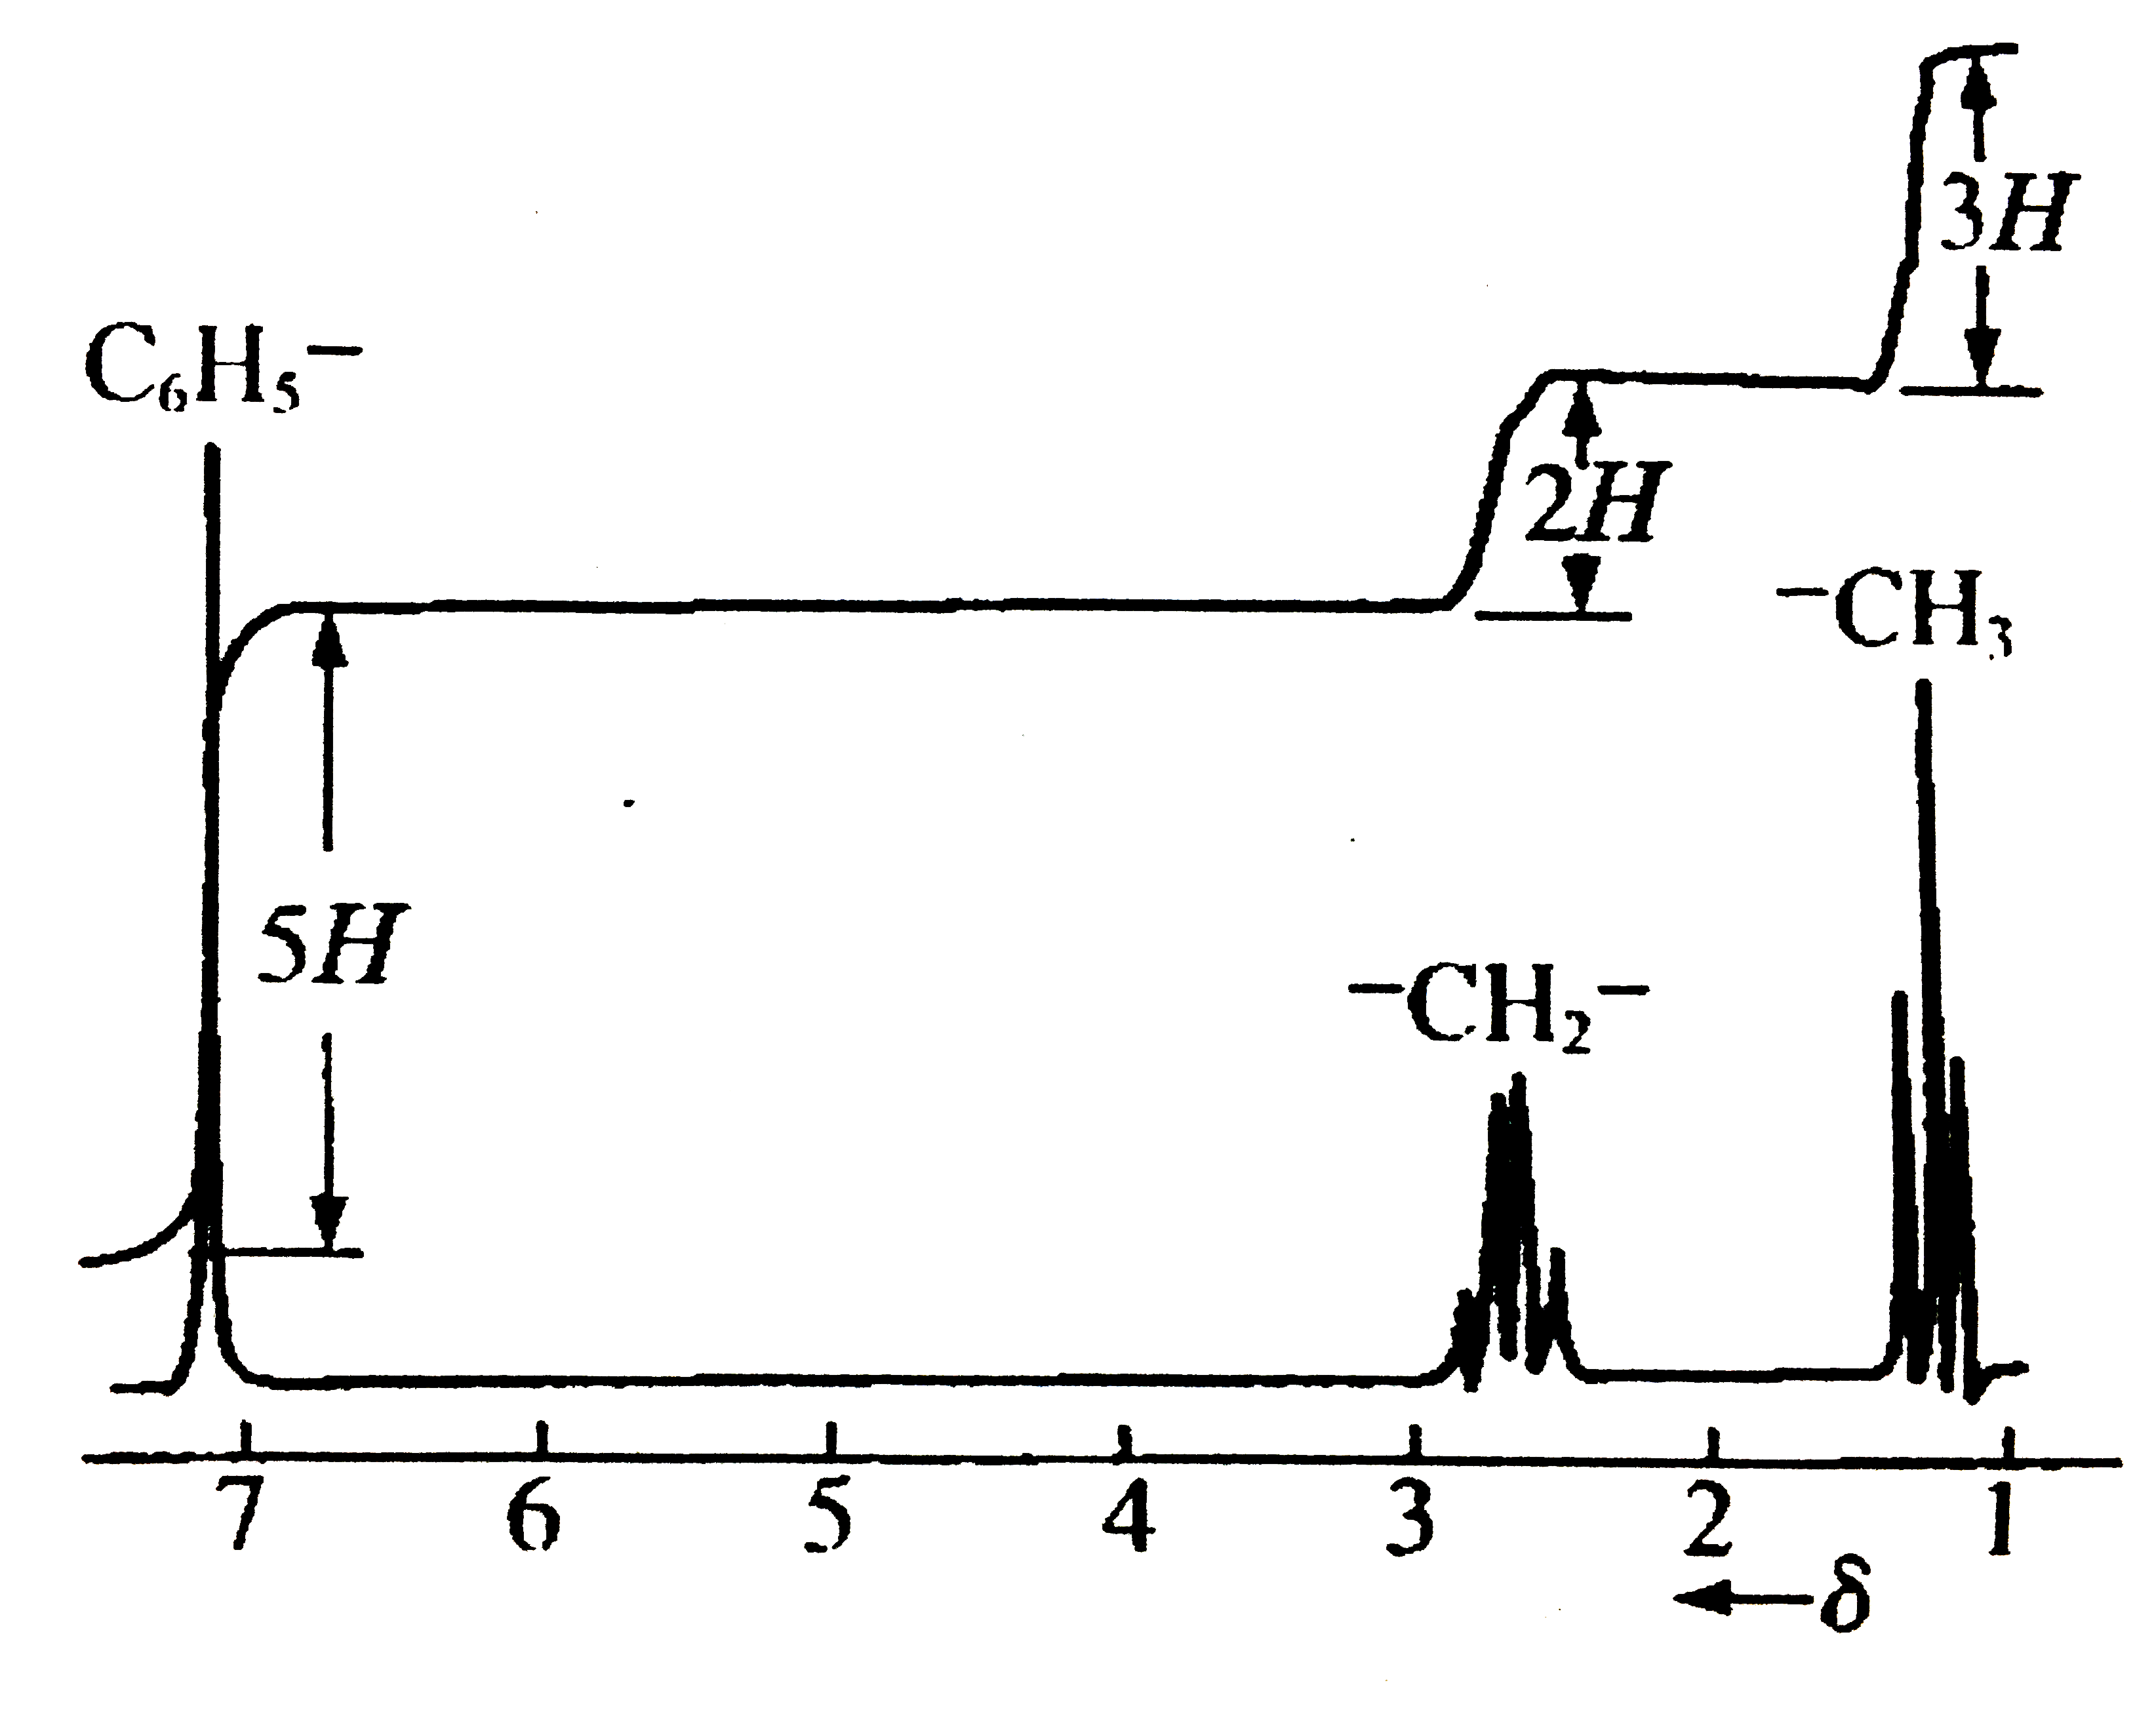
\includegraphics[width = 0.4\textwidth]{fig/3.png}\\
\caption{乙基苯(10\%CCl$_4$溶液)在100MHz时的核磁共振谱以及积分曲线}
\label{Fig3}
\end{figure}

由于化学位移差别范围很小,所以要精确测出其绝对值比较困难.一般都以相对数值来表示,测量精确度可在1Hz以内.测量时,以某一标准物质的共振峰为原点,然后测出各共振峰与原点的距离,再按下式定义计算出化学位移$\delta$值:

\begin{equation}\delta=\left[\frac{f_\text{样品}-f_\text{标准}}{f_\text{标准}}\right]\times 10^6=\left[\frac{H_\text{样品}-H_\text{标准}}{H_\text{标准}}\right]\times 10^6\end{equation}

式中,乘以$10^6$是为了使$\delta$所得数字易读易写.为此,通常把ppm(part per million的缩写,意思是百万分之一)作为$\delta$值的单位.对于60MHz的仪器,1ppm的宽度相当于频率改变60Hz.

\begin{figure}[H]
\centering
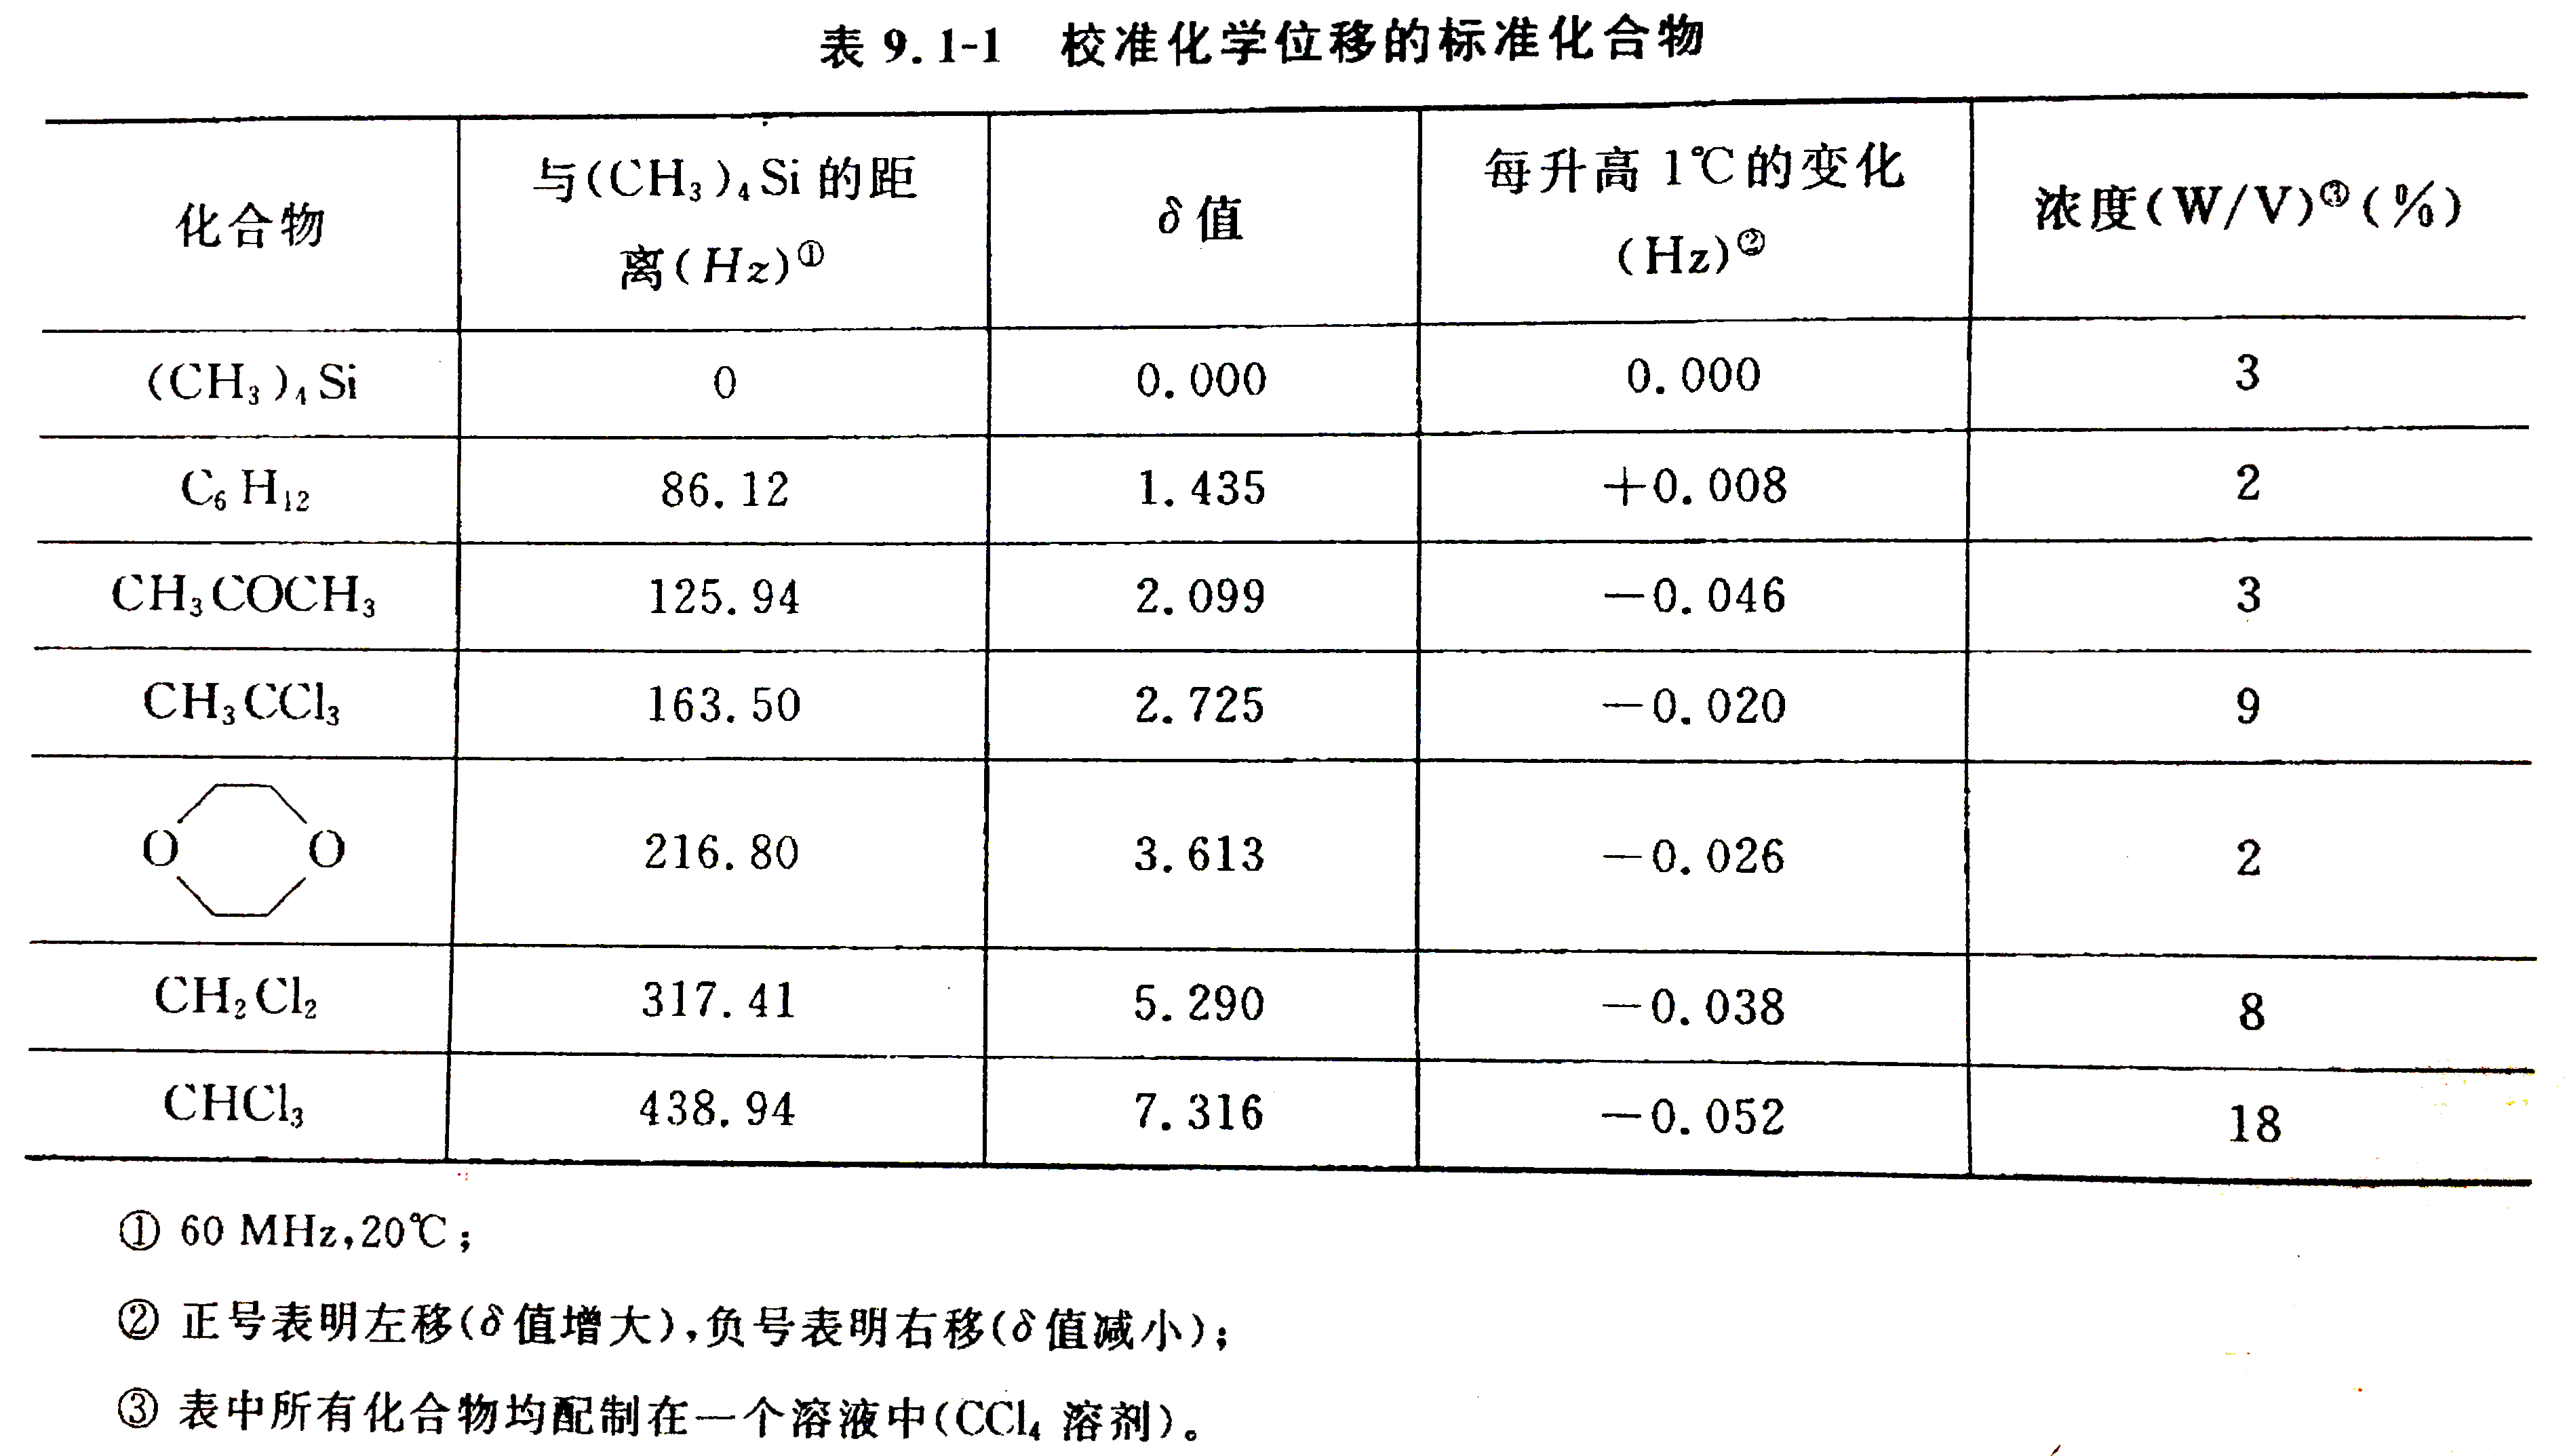
\includegraphics[width = 0.7\textwidth]{fig/4.png}\\
\caption{校准化学位移的标准化合物}
\label{Tab1}
\end{figure}

一般认定,标准样品四甲基硅$(\text{CH}_3)_4\text{Si}$的共振峰所在位置为$\delta$=0.它的共振峰只有一个单峰,且位于高场范围很容易识别.这种物质化学上惰性很大,它的12个质子呈球形分布,因此是各向同性的.它的共振磁场或共振频率随温度的变化很小.它的沸点为27$^\circ$C,易挥发,这有利于回收样品.此外,它易于和许多有机溶剂混溶.人们规定,在四甲基硅峰左边的$\delta$值为正,位于其右边的峰$\delta$值为负.

化学位移本身的校准常采用由几种化合物所组成的标准混合物,它们按表\ref{Tab1}的浓度配比封在一根玻璃管内供常规应用.

\subsubsection{耦合常数}

上面讨论的化学位移主要是考虑核磁的核外电子环境.实际上,同一分子内部的核磁间的相互作用不可忽略.虽然它不会影响化学位移,但对核磁共振谱的峰形有重大影响.例如图\ref{Fig3}中的甲基峰($-\text{CH}_3$)和亚甲基峰($-\text{CH}_2-$)分别为三重峰和四重峰,而不是单峰,这种现象就是由$-\text{CH}_3$和$-\text{CH}_2-$基团上的氢原子核之间的相互作用引起的.这种原子核之间的相互作用称为自旋耦合,由其引起的共振谱线增多的现象称为自旋分裂.

原子核间的自旋耦合是通过成键电子传递的.其主要机制是费米接触机制.设同一分子内有两个氢核$X$和$Y$,若两核之间无自旋耦合,则$Y$核只有一种跃迁存在,即$Y\left(+\frac{1}{2}\right)\to Y\left(-\frac{1}{2}\right)$.若两核之间有自旋耦合,且假定$X$核自旋为$+\frac{1}{2}$,则靠近它的电子自旋必定为$-\frac{1}{2}$ (核自旋极化电子自旋).按泡利原理,轨道上另一成键电子自旋必为$+\frac{1}{2}$.因此,只有当$Y$核自旋为$-\frac{1}{2}$时,这第二个成键电子才和$Y$核占据空间同一点.可以看出,$X\left(+\frac{1}{2}\right)$和$Y\left(-\frac{1}{2}\right)$使系统势能降低,而$X\left(+\frac{1}{2}\right)$和$Y\left(+\frac{1}{2}\right)$使系统势能升高.同样,对$X\left(-\frac{1}{2}\right)$核也可作类似分析,即$X\left(-\frac{1}{2}\right)$和$Y\left(+\frac{1}{2}\right)$使系统势能降低,而$X\left(-\frac{1}{2}\right)$和$Y\left(-\frac{1}{2}\right)$使系统势能升高.最后,由于$X$核的存在和它与$Y$核的自旋耦合,导致$Y$核有两种跃迁:$X$核自旋分别为$+\frac{1}{2}$和$-\frac{1}{2}$时,$Y\left(+\frac{1}{2}\right)\to Y\left(-\frac{1}{2}\right)$.这两种不同跃迁的能量差叫作耦合常数.

耦合常数是表征自旋耦合强弱的特征量.用$J$表示,单位为赫兹.耦合常数的大小与外加磁场无关.其值可正可负.但从核磁共振图谱,只能根据共振峰分裂后峰一峰之间的距离求出耦合常数,但无法确定其正负符号.

作为一个例子,我们简要讨论一下图\ref{Fig3}中的$-\text{CH}_3$共振峰为什么是三重峰而不是单峰.我们已经知道,氢原子核在磁场中有平行和反平行于磁场两种取向,这里分别用$\uparrow$和$\downarrow$代表$m=+\frac{1}{2}$和$m=-\frac{1}{2}$,则乙基苯的$-\text{CH}_2-$基团中的两个氢核的取向共有三种排列方式,即(1) $\uparrow\uparrow$;(2) $\uparrow\downarrow$或$\downarrow\uparrow$;(3) $\downarrow\downarrow$.因而,可产生三种不同的局部磁场作用于$-\text{CH}_3$基团上,从而使$-\text{CH}_3$的共振峰分裂为三,其高度比为1:2:1(因自旋相反的情况有两种排列方式,所以高度比例为2).

自旋分裂服从$n+1$律.该规律指出,当某基团上的氢有$n$个相邻的氢处在不同的环境中时,例如有一种环境的氢为$n$个,另一种环境的氢为$n'$个,则该基团氢应显示的核磁共振峰的数目为$(n+1)(n'+1)$个.由$n+1$律所得的复峰,其强度比例分别为1:1(二重峰)、1:2:1(三重峰)、1:3:3:1(四重峰)、1:4:6:4:1(五重峰)等,比例数字是由$(a+b)^n$进行级数展开后各项的系数决定.上例中,$-\text{CH}_2-$峰的自旋分裂是服从$n+1$律的.因为与它相邻的$-\text{CH}_2-$基含有两个氢,所以它会显示三个峰.

一般来说,按$n+1$律来估计耦合常数的$n+1$律方法叫作一级分析,按$n+1$律分裂的图谱称为一级图谱.应该指出,$n+1$律只是一个近似规律,实际得到的共振谱复峰与强度比并不严格按$n+1$律所预言.往往可看到对称的分裂峰高并不相等.实际分析图谱时,还常常必须考虑精细结构及二级分裂.

\begin{figure}[H]
\centering
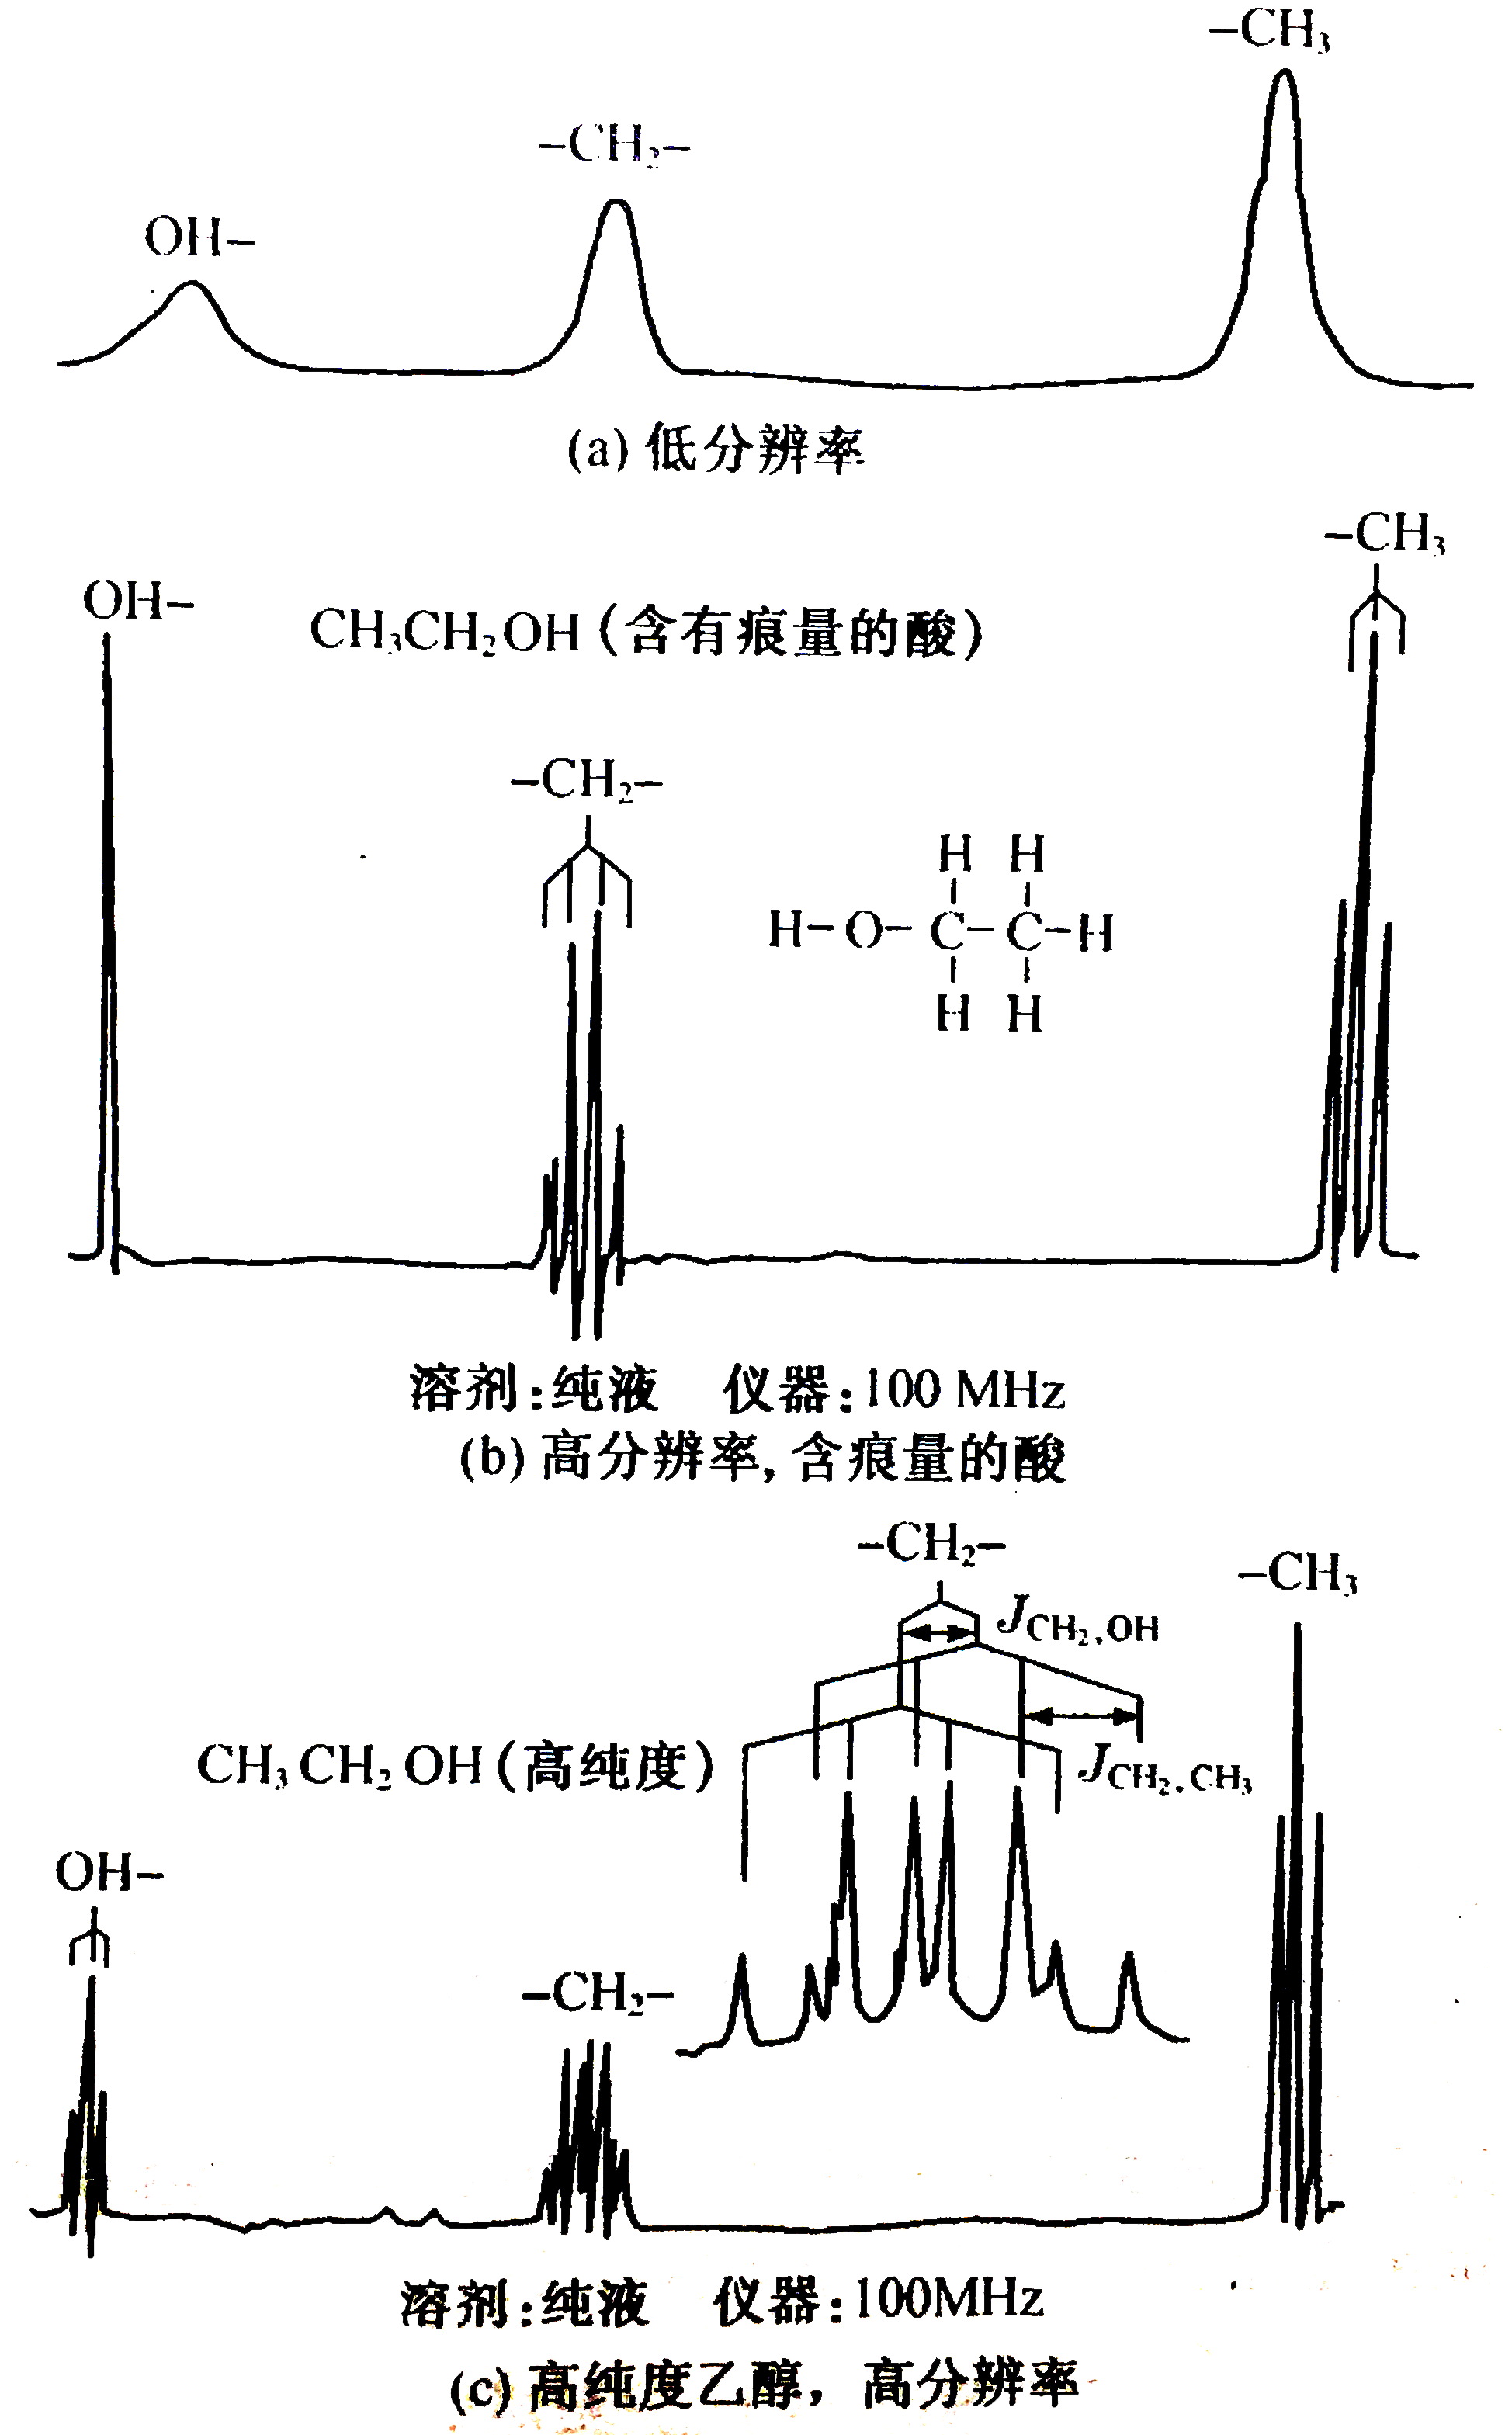
\includegraphics[height = 0.8\textheight]{fig/5.png}\\
\caption{乙醇的核磁共振氢谱}
\label{Fig4}
\end{figure}

图\ref{Fig4}示出了乙醇的核磁共振峰.图\ref{Fig4}(a)是低分辨率下的图谱,其中三个峰的面积之比为1:2:3,因而分别属于$\text{OH}-$,$-\text{CH}_2-$,$-\text{CH}_3$基团.图\ref{Fig4}(b)是分辨率提高后的图谱.此时,各组峰的面积之比仍为1:2:3,但$-\text{CH}_2-$,$-\text{CH}_3$基团峰是复峰,分别为四重峰和三重峰,遵守$n+1$律.然而,由于样品中包含了痕量酸,酸根离子以杂质的形式散布在氢核的周围,加强了自旋-晶格相互作用,造成能最交换速度加快,使$\text{OH}-$基团峰变成单峰,$\text{OH}-$和$-\text{CH}_2-$基团之问的峰的分裂不再遵守$n+1$律.若采用分析纯乙醇,则$\text{OH}-$峰也将变为复峰,如图\ref{Fig4}(c)所示,这时,各基团氢核共振峰相互之间由于自旋-自旋親合所造成的峰的分裂完全遵守$n+1$律.

\subsection{“磁等价”氢核的概念}

分子中若有一组氢核的化学位移相同,而对组外的任何一个氢核只有一种耦合常数,则这组氢核就被称为“磁等价”或简称“等价”.等价氢核之间虽然也有耦合(甚至耦合常数可能很大),但对共振谱不会发生任何影响.

例如在图\ref{Fig3}和图\ref{Fig4}中,甲基$-\text{CH}_3$的三个氢核的化学位移相同,但对外都只有一种耦合常数,所以甲基氢峰仅被“近邻”次甲基的氢所分裂,而亚甲基$-\text{CH}_2-$本身三个氢并不相互分裂.

\section{注意事项}
高分辨核磁共振仪是一台精密仪器,操作时应该十分小心.样品管放入磁场以前,先要放入量规孔中,调整好转子下沿与样品管底部的距离,确保样品进入磁场均匀区内.因为量规孔较小,而样品管壁又很薄,所以将样品管插人量规孔时要细心,以免样品管破损.

\section{实验内容}
画出各样品的核磁共振谱,计算化学位移和耦合常数。

\newpage

\section{实验数据}
\subsection{核磁共振谱}
\subsubsection{分析纯乙醇}
分析纯乙醇的核磁共振谱及化学位移和积分曲线如图(\ref{1OH} - \ref{1Integral})所示。
\begin{figure}[!h]
\centering
\includegraphics[width=12cm]{../data/1OH.jpg}\\
\caption{-OH核磁共振谱}\label{1OH}
\end{figure}
\begin{figure}[!h]
\centering
\includegraphics[width=12cm]{../data/1CH2.jpg}\\
\caption{-CH$_2$-核磁共振谱}\label{1CH2}
\end{figure}
\begin{figure}[!h]
\centering
\includegraphics[width=12cm]{../data/1CH3.jpg}\\
\caption{-CH$_3$核磁共振谱}\label{1CH3}
\end{figure}
\begin{figure}[!h]
\centering
\includegraphics[width=12cm]{../data/1Integral.jpg}\\
\caption{核磁共振谱的积分曲线}\label{1Integral}
\end{figure}

从积分曲线可知三种基团的峰的面积比为
\begin{equation*}
-OH : -CH_2 : -CH_3 = 1 : 2.12 : 3.27
\end{equation*}

\newpage
\subsubsection{含痕量硝酸的乙醇}
含痕量硝酸的乙醇的核磁共振谱及化学位移和积分曲线如图(\ref{2OH} - \ref{2Integral})所示。
\begin{figure}[!h]
\centering
\includegraphics[width=12cm]{../data/2OH.jpg}\\
\caption{-OH核磁共振谱}\label{2OH}
\end{figure}
\begin{figure}[!h]
\centering
\includegraphics[width=12cm]{../data/2CH2.jpg}\\
\caption{-CH$_2$-核磁共振谱}\label{2CH2}
\end{figure}
\begin{figure}[!h]
\centering
\includegraphics[width=12cm]{../data/2CH3.jpg}\\
\caption{-CH$_3$核磁共振谱}\label{2CH3}
\end{figure}
\begin{figure}[!h]
\centering
\includegraphics[width=12cm]{../data/2Integral.jpg}\\
\caption{核磁共振谱的积分曲线}\label{2Integral}
\end{figure}

从积分曲线可知三种基团的峰的面积比为
\begin{equation*}
-OH : -CH_2 : -CH_3 = 1 : 1.7 : 2.49
\end{equation*}

\newpage
\subsubsection{标准管}
标准管的核磁共振谱如图(\ref{3standard})所示。其各组分的化学位移数值与理论值的对比如表(\ref{table1})所示。

\begin{table}[!h]
\centering
\caption{标准管化学位移}
\label{table1}
\begin{tabular}{|c|c|c|c|}
\hline
组分 & 实验值  & 理论值   & 误差      \\ \hline
$C_6H_{12}$   & 1.43 & 1.435 & -0.35\% \\ \hline
$CH_3COCH_3$   & 2.11 & 2.099 & 0.52\%  \\ \hline
$CH_3CCl$   & 2.73 & 2.725 & 0.18\%  \\ \hline
1,4-二氧六环   & 3.62 & 3.613 & 0.19\%  \\ \hline
$CH_2Cl_2$   & 5.30 & 5.290 & 0.19\%  \\ \hline
$CHCl_3$   & 7.33 & 7.316 & 0.19\%  \\ \hline
\end{tabular}
\end{table}

\begin{figure}[!h]
\centering
\includegraphics[width=12cm]{../data/3standard.jpg}\\
\caption{标准管的核磁共振谱}\label{3standard}
\end{figure}

\newpage
\subsection{耦合常数}
实验所用的核磁共振仪的发生频率为$f_0 = $59.3MHz。四个耦合常数如下:
\begin{enumerate}
\item $J_{CH_2,CH_3}$\\
$$J_{CH_2,CH_3} = \cfrac{(2.56-2.33)+(2.45-2.21)}{4}\times f_0 \approx 7.00Hz$$
\item $J_{CH_3,CH_2}$\\
$$J_{CH_3,CH_2} = \cfrac{0.113 - (-0.125)}{2}\times f_0 \approx 7.06Hz$$
\item $J_{OH,CH_2}$\\
$$J_{OH,CH_2} = \cfrac{4.13 - 3.96}{2}\times f_0 \approx 5.04Hz$$
\item $J_{CH_2,OH}$\\
\begin{eqnarray*}
%\begin{split*}
J_{CH_2,OH} &=&
   \left(\frac{2.41+2.30}{2} - \frac{2.33+2.21}{2}\right)\times\frac13\times f_0  \\
 &+& \left(\frac{2.53+2.41}{2} - \frac{2.45+2.33}{2}\right)\times\frac13\times f_0  \\
 &+& \left(\frac{2.65+2.53}{2} - \frac{2.56+2.45}{2}\right)\times\frac13\times f_0 \\
 &\approx& 4.92Hz
%\end{split*}
\end{eqnarray*}
\end{enumerate}

\section{思考题}
\subsection{何谓化学位移和耦合常数?怎样从所画出的核磁共振谱上求出这两个参数?}
\subsection{调整核磁共振谱时,如何判断相位与分辨率调整得正确与否?}
\subsection{为什么在高分辨率下含痕量酸的乙醇的$\text{OH}-$峰是单峰和$-\text{CH}_2-$峰是四重峰?为什么在很纯的乙醇时,$\text{OH}-$峰变成三重峰,而$-\text{CH}_2-$峰则分裂成八个峰?}

\nocite{jiaocai}
\bibliography{ref}
\end{document}